\section{Family Ties Between 1523 and 1680}
During the time period between 1523 and 1680 there were 257 men active in the Council of the Realm. As discussed earlier in subsection \ref{councilofrealm} the Council consisted mostly of men with noble background. To quantify this: according to the dataset 236 of the 257 councillors (91.8\%) were part of the ancient nobility (\textit{uradel}), and only approximately 5\% were of unknown or ignoble background, most of the time bishops or other clerics.  

\begin{table}
	\caption[Absolute amount in different ranks]{Absolute amount in different ranks (Data by \cite{councillorsDS}, statistics by author)}
	\centering
	\begin{tabular}{cccccc}
		\hline
		Commoner & Ennobled & Estate unknown & Unknown & Ancient nobility & \\
		\hline
		5 & 8 & 7 & 1 & 236 & = 257 \\
		\hline
	\end{tabular}
	\caption{Proportional amount in different ranks}
	\centering
	\begin{tabular}{cccccc}
		\hline
	    Commoner & Ennobled & Estate unknown & Unknown & Ancient nobility & \\
	    \hline
	    1.9 & 3.1 & 2.7 & 0.3 & 91.8 & $\approx$ \% \\
	\end{tabular}
\end{table}

The kingdom of Sweden was ruled by nine monarchs: Gustavus Vasa (1523-1560), Eric XIV (1560-1568), John III (1568-1592), Sigismund (1592-1599), Charles IX (1599-1611), Gustavus Adolphus (1611-1632), Christina (1644-1654), Carl X Gustav (1654-1660) and Carles XI (1672-1697), and two regnant from 1632 to 1644 and from 1660 to 1672 during the time period.\footcite[p. 11]{lappalainen06} The amount of councillors appointed by each monarch\footnote{Calculated with a R script. To avoid the script duplicating the years that the monach changed, the beginning of each reign is adjusted, the actual year + 1. E. g. Eric XIV's reign is calculated 1561-1568, the actual being 1560-1668. This may cause slight inaccuracy.} or regnant varied from none to 56. Yet, 13 councillors present in the dataset had been appointed before the reign of Gustavus Vasa.

The monarchs who appointed the most councillors were Gustavus Vasa (56) and queen Christina (45). The large number of councillors appointed by Gustavus Vasa may be explained by the sheer length of his reign. He ruled Sweden for 37 years, whereas all of the other monarchs ruled less than 20 years. Also the religious Reformation was performed during his reign. The bishops and clerics that lost their position in the Council were replaced by noblemen chosen by the king.\footcite[p. 74.]{pSuurvalta} As queen Christina ruled only for ten years, the exceptionally high number on her reign is interesting. Therefore, her reign will be discussed in greater detail in subsection \ref{christina}. 

However, the king who appointed no new councillors was the son of king John III: Sigismund (1566-1632). He was both the king of Poland and Sweden forming a personal union between the two countries. Why king Sigismud did not appoint any new councillors? 

Sigismund was the son of king John III and his wife Catarina Jagellonica (1526-1583). Catarina Jagellonica was a descendant of the European royalty, remarkably she was the sister of the king of Poland, and a daughter of Milan princess Bona Sforza (1494-1557)\footnote{For more info see e. g. \cite{bona_sforza}.}. Sigismund was born in 20th of June 1566 while his parents were imprisoned by John's brother king Eric XIV in the Gripsholm castle. Due his mother's position and faith, Sigismund was raised as a Catholic.\footcite[p. 27, 47.]{lappalainen09}

Sigismund was elected to be the king of Poland in 1587. After his father's death in 1593 Sigismund also inherited the throne of Sweden. Sigismund's enforcement of the Catholic faith caused fear and suspicion amongst his Swedish subjects, and the interactions between the parties have been described as hiddenly antagonistic. The tense situation culminated in a civil war won by the duke Charles in 1599 (or 1604), as Sigismund lost his kingship of Sweden in 1599.\footcites[pp. 49-52, 78-81, 100-111, 259-267.]{lappalainen09}{sbl_sigismund} Even though he was not particularly popular in Poland either, Sigismund remained the king till his death in 1632. The Polish crown was inherited by his oldest son Vladislav.\footcite{sbl_sigismund}

It seems that the answer on why Sigismund appointed no councillors lies in the overall mistrust between the king and his subjects. Sigismund was not a particularly popular king amongst the Swedish nobility, and vice versa, he did not trust his councils in Sweden. 

\begin{figure}
	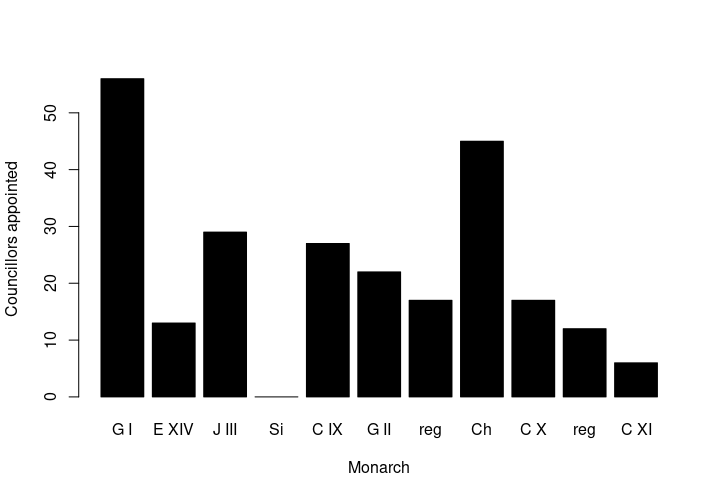
\includegraphics[scale=0.6]{councillorspermonarch.png}
	\centering
	\caption[Number of councillors appointed by each ruler between 1523-1680] {Number of councillors appointed by each monarch or regnant from 1523 to 1680. (Data by \cite{councillorsDS}, figure by author) From left to right G I: Gustavus I Vasa (1523-1560), E XIV: Eric XIV (1560-1568), J III: John III (1568-1592), Si: Sigismund (1592-1599), C IX: Charles IX (1599-1611), G II: Gustavus Adolphus (1611-1632), reg: regnant (1632-1644), Ch: Christina (1644-1654), C X: Carl X Gustav (1654-1660), reg: regnant (1660-1672) and C XI: Carles XI (1672-1697).}
	\centering
\end{figure}

All of the councillors active between 1523 and 1680 are represented in a graph of 257 nodes and 362 edges, with self loops and parallel edges removed. The number of edges exceeds the number of nodes which means that theoretically all of the nodes could be linked to one another. Although, the edges are not distributed that way. Some of the nodes are linked to more than one other node, but some isolated nodes are indeed present. The average degree of the graph is 2.817 $\approx$ 2.8 meaning that councillors typically had 2 or 3 direct relations to another members of the Council.

The graph density is 0.011. In the mathematical definition the graph is sparse (scale from 0 to 1). However, interpretation in practical sense is not that straightforward. Having a completely dense social network, meaning that every node is directly linked to each other, is almost impossible. In this context it would mean, that each councillor is a direct relative through blood or marriage to each other, which would be weird to say at least. Further, taking the dimension of time into account, the mathematical interpretation would be even more nonsensical: how a nobleman appointed to the council in the 1670's could be directly linked to a bishop died in 1530's. 

The question whether or not the councillors were highly linked to each other is more of a qualitative one. In the context of early modern institution, how we define a highly linked or even nepotistic institution? Probably the graph density has more explanatory value as a parameter to be compared between graphs collected from other contemporary communities.

Even so, the proportion of the nodes with at least one connection in the graph is $224/257 \approx 0.8715$ Which means that between 1520 and 1680 the probability of a councillor being related to someone else in the Council is $\approx$ 87\%. In that sense the councillors can be considered highly networked.

Another interesting finding are the nodes with the highest and lowest degree. Maybe the most eclectic and fascinating group is the isolated nodes. There are 33 isolated nodes meaning that 33 councillors did not have any family ties within the Council. Some of them are members of the nobility with family ties to councillors active prior the beginning year of the dataset, so the connections are excluded from this graph. These are for example: Ture Bengtsson Lilliesparre (id 127, died 1524) or Nils Olofsson Vinge (id 242, died 1529). Yet, some of the isolated nodes represent bishops and clerics like Magnus Sommar (id 186, died by 1542) or Ingemar Petri (162, died 1530) present in the Council before the religious Reformation. 

Besides that, the isolated nodes also reveal something about the international relationships during the time period. For example a teacher from France Dionysius Beurraeus (id 12, 1507-1567) or a Scottish baron Robert Douglas (id 58, 1611-1662) can be found. Dionysius Beurraeus came to Sweden invited by Conrad von Pyhy (id 168, circa 1500-1553) in 1543. Due his knowledge in mathematics and medicine Beurraeus took part in the upbringing and teaching Gustav Vasa's sons in the Swedish court. He became close with the king Eric XIV and was appointed to the Council in 1562. However, his life ended dramatically only five years later, in 1567 in the violent outburst of the unstable king. The act of violence is called \textit{Sturemorden} (murder of Sture family).\footcite{sbl_DB}   

As discussed in the end of subsection \ref{sources}, it is hard to say for sure, whether or not Robert Douglas (id 58) was in fact a member of the Council, but regardless of his official position as a councillor, he held a significant standing amongst the Swedish aristocracy in the mid-17 century. Also the famous German born chancellor Conrad von Pyhy (id 168) is represented as an isolated node. During his stay in Sweden von Pyhy had a significant impact on the politics of Gustavus Vasa.\footcite[pp. 81-83.]{pSuurvalta} This means that as a merited foreigner one could make their way up to the Swedish Council of the Realm.

On the contrary, the nodes with the highest degree ($\geq$ 5) are of councillors who are part of the old well established aristocratic families like De la Gardie, Oxentierna, Gyllenstierna, Bielke, Stenbock, Sparre and Ribbing. Also Finnish families of Horn and Kurck can be found. That in itself ties to the previously known fact that the aristocratic families had a remarkable stance in the negotiations and politics of the Swedish kingdom.

To focus more on the temporal dimension of the graph, I decided to divide the dataset in half. As seen in Figure \ref{fig:peryear} the most intuitive point to do the division is between years 1600 and 1601. By year 1601 duke Charles had won the civil war against king Sigismund and he practically decimated the Council of the Realm while eliminating the noblemen loyal to the former king. However, by 1602 he had to appoint 15 new councillors in order to manage the growing number of tasks in diplomacy and administration.\footnote{See subsection \ref{councilofrealm}} By coincidence, year 1601 also divides the time range of the dataset almost in half. The first graph depicts the network prior to year 1600 and the latter one post year 1601, so both of these represent the family ties accumulated approximately for 80 years.

\subsection{Prior to Year 1600}
The graph depicts the family links within the Council during most of the 16th century. It consist of 111 nodes and 92 edges. In this case the number of edges subceeds the number of nodes meaning that at least some isolated nodes must be present. 

The average degree in this graph is 1.658 $\approx$ 1.7, meaning that typically councillors were directly related to one or two other members. The number is smaller than in the larger graph. However, it can be partly explained by the shorter time range, simply the family networks had not have enough time to accumulate. Thereafter, the closest comparison is the graph of councillors family ties post 1601, which will be discussed later.

The graph density is 0.015, although, comparing that to the larger graph is not that straightforward. The amount of nodes having at least one connection is $85/111 \approx 0.765$ meaning that the probability of councillors to be linked at least one other member is $\approx 77\%$. That is 10 percentage points smaller than in the larger graph. Even though this prior to year 1600 graph is not directly comparable with the larger graph, it indicates that the family links in the 16th century were more sparse.

The amount of isolated nodes is significant: 26–whereas in the larger graph it was 33. The fact that all of the bishops and clerics must be present in this graph partly explains this. Limiting the time range also breaks some of the existing links, so for example, Pontus De la Gardie seems to be without any connections in that graph, even though his descendants were remarkably woven into the networks of Swedish aristocracy. Taking these factors into account, still the relatively high number of isolated nodes may suggest the relatively high number of incomers and larger social mobility in general.

The nodes with highest degree ($\geq$ 4) were of the remarkable noble families such as Bielke and Stenbock, however the Bååt family is more apparent in this particular graph than in the larger one or any of the latter ones. Why did the family name disappear? According to Swedish \textit{Riddarhuset} -website the family was extinct in the 17th century (extinct on the male line \textit{Utdöd svärdssidan} in 24.12.1654 and extinct on the female line \textit{Utdöd spinnsidan}\footnote{Sword and "spinn" $\rightarrow$ spindle (tool for making yarn).} in 1698 or 1699).\footcite{riddarhuset} It seems that the family was indeed in the process of dying down during the time period, as usually happened to the noble houses of the 17th century.\footnote{See subsection \ref{background}}

\subsubsection{The Last Man Standing: Nils Gyllenstierna}
The latter half of the 16th century and especially the turn of the 17th century was politically turbulent time in the kingdom of Sweden. The latter half of the 16th century being affected by the rivalry between the sons of Gustavus Vasa which culminated in the civil war during the 1590's. The battle between king Sigismund and duke Charles was won by duke Charles, who later directed his spite upon the Council of the Realm. Many of the councillors were executed or fled Sweden. Despite that the Council was almost fully devastated in 1601, one councillor was left behind: Nils Göransson Gyllenstierna (id 91, 1526-1601).

Due to these circumstances, Nils Gyllenstierna had an exceptional political career. He was a nobleman born in 1526 to a family with three generations of councillors. In his youth he studied in the university of Wittenberg. In autumn 1560 he was given the title of a chancellor and appointed to the Council of the Realm by Eric XIV, at the age of 35.\footcite{sbl_nils_gyllenstierna} 

He did outlive the rivalries of the Gustavus Vasa's sons, yet only slightly. In year 1597 he was already elderly, ill and weak, but almost got executed by the command of Duke Charles.\footcite[pp. 205-206.]{lappalainen09} He was mostly able to stay away from the heat of the conflicts between the Council and duke Charles, and in the late 1590's he declined the invitations to the Diet and the Council meetings, by claiming his old age.\footcite{sbl_nils_gyllenstierna} When he died of natural causes in 1601 at the age of 75, he had served a total of 41 years in the Council.\footcite{councillorsDS} Somehow he he had been able to keep his position throughout all of the Gustavus Vasa's sons reigns. Retroactively it seems that his tactic was not to take sides, and not to be in the wrong place at the wrong time.

Nils Göransson Gyllenstierna (id 91) had a significant amount of councillors directly related to him. His father Göran Eriksson Gyllenstierna (id 88, 1498-1575) and son Jöran Nilsson Gyllenstierna (id 86, 1575-1618) were in the Council. His father-in-law Axel Eriksson Bielke (id 13, circa 1500-1559) was a councillor. He had also four sons-in-law in the Council. Overall, he had seven direct connections, and several indirect ones. The degree of the node representing him was seven, and the node was amongst the 8.17\% which had degree of $\geq 7$. If the indirect connections are counted to the distance of three\footnote{Meaning that the node's neighbors, neighbors' neighbors and neighbors' neighbors' neighbors are counted. See section \ref{network}.}, the indirect connections consists of 72 nodes. Meaning $\approx 28 \%$ of the dataset's councillors are within three connections from Nils Göransson Gyllenstierna.

The last councillor to be executed in Sweden was Hogenskild Nilsson Bielke (id 16). He was born in 1538, and appointed to the Council by king Eric XIV in 1562 at the age of 24.\footcites[p. 58.]{HakanenAKoskinen2017}{councillorsDS} In his youth he studied in Finnish town of Turku and later in famous European universities, and was influenced by the teachings of the Finnish reformer Mikael Agricola. In 1569 he married Anna Sture (1541-1595) the daughter of Svante Stensson Sture(id 217, 1517-1567).\footcite{sbl_bielke_hongeskild} Due his exceptional education has been described as the spokesperson of the old nobility.\footcite[p. 55.]{lappalainen09}

In year 1600 he became suspected of treason by duke Charles and was imprisoned in Linköping. The legal process took five years, but consequently he was sentenced to death of high treason, and executed in 3rd of June 1605 at the age of 67.\footcite{sbl_bielke_hongeskild} All in all, he had served in the Council of the Realm for 36 years (being inactive for two years between 1590-1591).\footcite{councillorsDS}

Hogenskild Nilsson Bielke does not seem to have had a firm network of related councillors behind him, that does not mean that he did not have a network of supporters and allies, which he most likely had. His only direct connection on the graph was to his father-in-law Svante Stensson Sture (id 217). In fact, Svante Stensson Sture with his two sons Nils and Erik Sture were tragically killed–directly or indirectly–on the hands of Eric XIV in 1567. Besides Svante Sture and his sons, the violent act of \textit{Sturemorden} claimed at least three more victims, Abraham Gustavsson Stenbock, Ivar Ivarsson Liljeörn and Eric's own teacher Dionysius Beurræus (id 12). Svante Sturesson Sture was buried together with his two sons.\footcite{sbl_svante_sture} This means that both Hogenskild Nilsson Bielke and Svante Stensson Sture were put to death by Gustav Vasa's sons.

\subsection{Post Duke Charles' Revenge}
Practically, this graph begins from the year 1602 when duke Charles had to appoint 15 new councillors and the Council of the Realm was re-established. The graph consists of 146 nodes and 184 edges, now the number of edges exceeds the number of nodes. After 1601 (or 1602) the average degree of node is 2.251 $\approx$ 2.3, larger than the 1.7 prior to 1600. Also, visually the graph seems more dense. 

The number of isolated nodes is significantly lower: 16, compared to the 26 prior to 1600 or the 33 in the whole time period. Again it still must be remembered that limiting the time range cuts some family ties present in the dataset. Subsequently, the proportion of nodes with at least one edge is $130/146 \approx 0.89$, thereby, the probability of councillor having at least one direct relation in the Council was now $\approx 89\%$. That is 12 precentage points greater than the 77\% in the 16th century, and two precentage points greater then the 87\% from the whole time period.

\begin{table}
	\caption[Number of edges needed for different densities of network]{Number of edges needed for different densities of network. The observed numbers are bolded}
	\label{edges}
	\begin{tabular}{cccc}
		\hline
		&& Amount of possible edges & \\
		\hline
		Density & 32 896 (all) & 6 105 (prior to 1600) & 10 585 (post 1601) \\
		\hline 
		0.011 & \textbf{361.9} & 67.2 & 116.4 \\
		\hline
		0.015 & 493.5 & \textbf{91.6} & 158.8 \\
		\hline
		0.0174 & 572.4 & 106.2 & \textbf{184.2}\\
		\hline
	\end{tabular}
\end{table}

Also the density of this graph is the largest: 0.017. In prior to 1600 it was 0.015 and from the whole time period 0.011. To make the densities comparable to some degree, the amount of edges needed for different densities is counted in Table \ref{edges}. Still, the scale of the larger graph makes it hard to compare with the other graphs, so, I will focus on the two smaller ones. The graph prior to 1600 would need $\approx 14$ more edges to have the density of 0.017, whereas in the graph post 1601 the difference between the density of 0.015 and 0.017 is $\approx 26$. This behaviour is explained in the subsection \ref{network}. So, even though the time scale is similar (80 years), the density and the absolute amount of edges is different. This means that it can be argumented that the post 1601 graph is more dense than the one prior to 1600. 
 
One interesting isolated node is one representing Johan Adler Salvius (id 2, 1590-1652). Johan Salvius was of merchant background, he was orphaned and raised by the Bishop of Strängnäs. He got the change to study in the European universities and therefore landed a position in the Svea Royal Court (\textit{Svea hovrätt}). As a skilled officer he was noticed by king Gustav II Adolph, who later hired him as a diplomat. He was part of the Swedish delegation in the peace treaties of Westphalia in 1648, that ended the Thirty Years War in Europe.\footcite{marjomaa2000}

He was ennobled in 1629, and appointed to the Council of the Realm in 1648 by queen Christina despite the opposition provoked by his ignoble birth. To gain financial stability he had married a wealthy elderly widow in his youth. Nevertheless, the elderly lady happened to outlive her husband. Due this Johan Adler Salvius left no direct heirs, and the dispute over the inheritance of his massive property lasted until the 19th century.\footcite{marjomaa2000}

All in all, 17th century has been called in the previous literature "the Age of the Aristocracy", and the presented data seems to confirm the trend.\footcite{hakanenAndHaikari2020} It seems that the family affiliations became more prominent in the Council of the Realm, and important in general, during the 17th century. Similarly, the amount of incomers decreased, which implies the slowdown of social mobility.

\subsection{In the Court of Queen Christina}
\label{christina}
Queen Christina (1626-1689) was the daughter of the king Gustavus Adolphus and queen consort Maria Eleonora of Brandenburg (1599-1655). She inherited the throne at the age of 6, after her fathers sudden death in the battlefield in November 1632. Before she was declared an adult at the age of 18 in 1644, the kingdom was ruled by a regnant.\footcite[pp. 188-189, 288-289.]{lappalainen14} The reign and especially the personal life of queen Christina are fascinating chapters in the Swedish history, and she is the most researched monarch in the European history.\footcite[For more information see e.g. Peter Englund \textit{Silvermasken: en kort biografi över drottning Kristina} finnish version \textit{Kuningatar Kristiina}, or Marie-Louise Rodén \textit{Drottning Christina: en biografi}.]{makelaAlitaloEtAl2000}

During the time of Christina's birth the future of the inheritance of the Swedish throne was at stake. Cristina's grandfather Charles IX had claimed the crown from his nephew Sigismund in 1599 (or 1604) and left it to his son Gustav II Adolph.\footnote{See subsection \ref{councilofrealm}} In the case of Gustav II Adolph's death the chance of Sigismund reclaiming the kingdom was high. Gustav II Adolph needed a son. Due a series of misfortunes his and Maria Eleonora's only child surviving infancy was a girl: Christina. Christina was declared to be the rightful heir to the throne, and she was educated as a future ruler.\footcite[pp. 185-189.]{lappalainen14}

Although educated and skilled monarch, she provocated the Council of the Realm many times during her reign. Politics aside, she was not considered as a skilled ruler when it came to the economics, and she has said to spent fortunes on the lavish lifestyle on the court with her inner circle. Also her atypical behavior further fueled questions and rumors surrounding her persona.\footcite{makelaAlitaloEtAl2000}

She started preparing the abdication of the throne in the early 1650's, however, was forced to postpone the process by years. Officially she abdicated the throne in 6th of June 1654 in favor of her cousin Carl X Gustav (1622-1660), and left Sweden in 10th of June the same year. In 1655 she officially converted to Catholicism, and changed her name to Maria Christina Alexandra. She moved to Rome where she lived the rest of her life.\footcite{makelaAlitaloEtAl2000}

She came back to Stockholm accompanied by Italian court and a Catholic monk in 1660, and tried to reclaim the right to the inheritance of the Swedish throne. This caused concern amongst the monarch and the Council, who demanded her to reassure her renouncement of the crown. She left Sweden in 1661 and never returned. In Rome she was known for her support for the arts, theater and opera. She died in Rome in 1689. Queen Christina left behind an ambivalent legacy, particularly in Sweden she was heavily criticized on her choices.\footcite{makelaAlitaloEtAl2000}

In the early years of her reign she had to acquire the authority over the Council of the Realm. Due that Christina's father was frequently away from Sweden and the long period of the interregnum, the power of the Council had grown remarkably when Christina was enthroned. Contrary to the previous monarchs, she was forced to go for the Council to get counsel, yet, the situation did not stay that way for long.\footcite[p. 64.]{HakanenAKoskinen2017} In the words of Hakanen and Koskinen: 

\begin{quote}
	Christina played the high nobility at their own social network game rather than enter into open warfare with them. That is, she quickly created a large group of loyal supporters around her $\dots$\\
	(\cite[p. 64]{HakanenAKoskinen2017})
\end{quote}

Furthermore, she appointed many new councillors to dilute the power of the original Council. By the year 1654 she had appointed 45 new councillors.\footcite[p. 64.]{HakanenAKoskinen2017}

As queen Christina notoriously appointed councillors to dilute the power of the old Council, did she favor any age group, perhaps young educated noblemen? To give an indicative answer to this question, I calculated the summary statistics on the age distribution on the councillors appointed by Christina, and the same statistics on the age distribution from the whole dataset. As we can see from the Tables \ref{councillorsages} and \ref{agesByChristina} the councillors appointed by Christina were the same age-range as the councillors appointed by all of the monarchs. In fact, the distributions seems fairly similar. However, in the whole dataset N (the number of observations excluding missing values) is 200, whereas in the part appointed by Christina N is 44, meaning that the distributions are not fully comparable.

Typically the councillors were appointed in their late 30's (median 38, mean 39.6), also the councillors appointed by Christina were of similar age (median 37, mean 39.36). Overall, the youngest councillors appointed were only the age of 22 years. They were Sten Eriksson Lewenhaupt (Leijonhufvud) (id 118, 1518-1568), Per d.ä. Joakimsson Brahe (id 40, 1520-1590) and Gustaf Axelsson Baner (id 5, 1547-1600). The youngest councillors appointed by Christina were 25 years old Magnus Gabriel Jacobsson De la Gardie (id 56, 1622-1686) and Henrik Fransson von Thurn (id 221, 1628-1656).

The oldest councillor to be appointed was Måns Svensson Some (id 187, 1495-1571). He was appointed in the age of 74, and served only two years in the Council before his death in 1571. The oldest councillor appointed by Christina was Konrad Falkenberg (id 61, 1591-1654) in the age of 61. He was appointed in 1652, and coincidentally also he died two years after his appointment in 1654.

\begin{table}
	\caption[Summary statistics on the councillors ages of appointment]{Summary statistics on the councillors ages of appointment from the whole dataset (including the reign of Christina). NA meaning a missing value. N = 257 - 57 (Data from \cite{councillorsDS}, statistics by author)}
	\label{councillorsages}
	\centering
	\begin{tabular}{c c c c c c c}
		\hline
		Min. & 1st Qu. & Median & Mean & 3rd Qu. & Max. & NA's \\
		\hline
		22.0 & 33.0 & 38.0 & 39.6 & 45.0 & 74.0 & 57 \\
		\hline
	\end{tabular}
	
	\caption[Summary statistics on the councillors ages appointed by queen Christina]{Summary statistics on the ages of appointment from the councillors appointed by queen Christina. N = 45 - 1 (Data from \cite{councillorsDS}, statistics by author)}
	\label{agesByChristina}
	\centering
	\begin{tabular}{c c c c c c c}
		\hline
		Min. & 1st Qu. & Median & Mean & 3rd Qu. & Max. & NA's \\
		\hline
		25.00 & 32.75 & 37.00 & 39.36 & 45.75 & 61.00 & 1\\
		\hline
	\end{tabular}
\end{table}

The network of councillors appointed by queen Christina is displayed in Figure \ref{queenChristinaCouncillors}. As queen Christina's reign lasted for only ten years the graph is not comparable to the other larger graphs, despite that, it is interesting in its own right. The graph consist of 45 councillors, all of them which must have been close to queen Christina in one way or another.

\begin{figure}	
	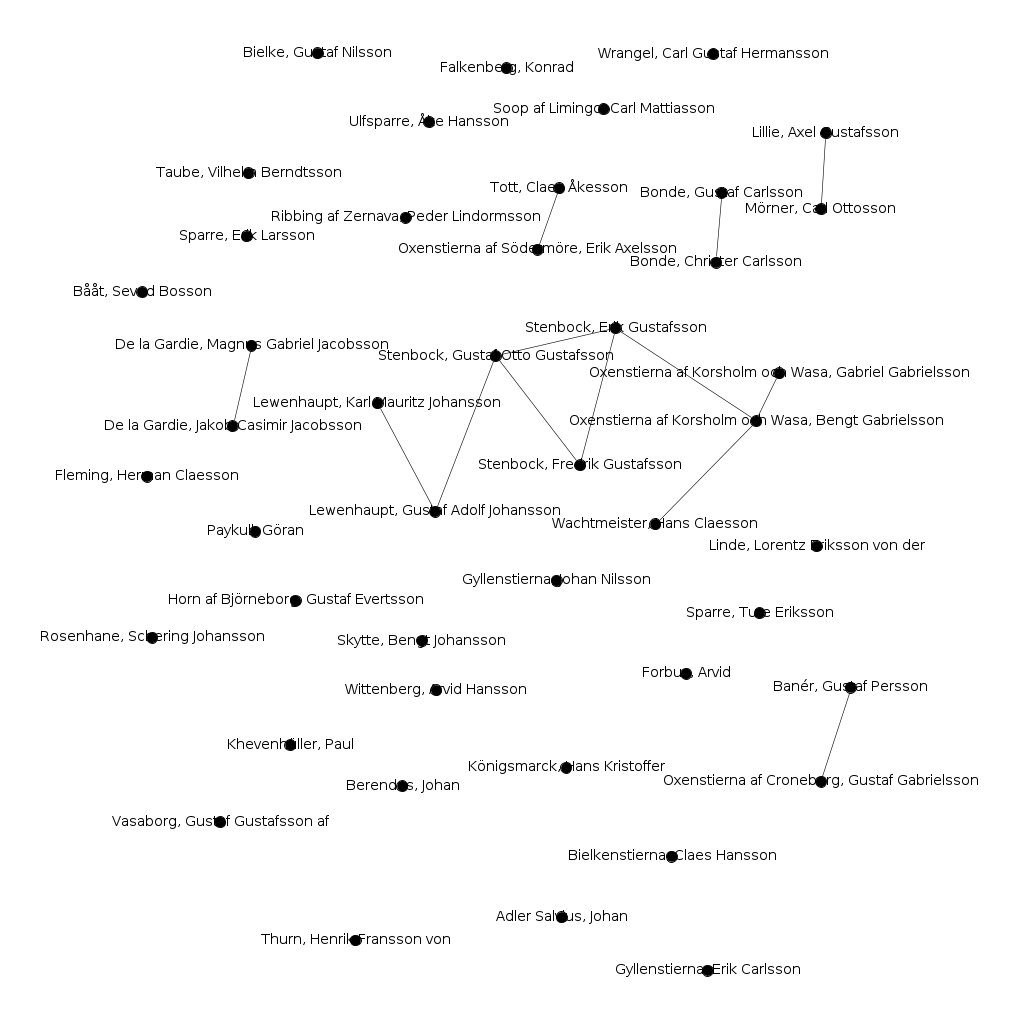
\includegraphics[width=\linewidth]{councillors_1644-1654.png}
	\caption[Councillors appointed by queen Christina]{A graph of councillors appointed by queen Christina between 1644 and 1654.(Data by \cite{councillorsDS}, graph by author)}
	\label{queenChristinaCouncillors}
	\centering
\end{figure}

Overall, the graph seems more like a list, but, an interestingly clustered pattern can be found in the middle of the network. Eight councillors: Karl Mauritz Johansson Lewenhaupt (id 125, 1620-1666), Gustaf Adolf Johansson Lewenhaupt (id 126, 1619-1656), Gustaf Otto Gustafsson Stenbock (id 207, 1614-1685), Fredrik Gustafssonare Stenbock (id 204, 1607-1642), Erik Gustafssonall Stenbock (id 202, 1612-1659), Bengt Gabrielsson Oxenstierna af Korsholm och Wasa (id 148, 1623-1702), Gabriel Gabrielsson Oxenstierna af Korsholm och Wasa (id 154, 1619-1672) and Hans Claesson Wachtmeister (id 240, 1609-1652) are all related to each other direclty or indirectly. 

This tightly woven network seems to concentrate around the two brothers Gustaf Otto Gustafsson (id 207) and Erik Gustafsson Stenbock (id 202). They were part of the mighty Stenbock family. Their father was a councillor Gustaf Eriksson Stenbock (id 205, 1575-1629) who's father (id 203) and grandfather (id 206) were also in the Council. The brothers were councillors in the fourth generation. 

Some other interesting individuals can be also found in the graph. Christina appointed his paternal half brother Gustaf Gustafsson af Vasaborg (id 241, 1616-1653)–Gustavus Adolphus' illegitimate son–to the Council on 5th of September 1646. Also the diplomat and nobleman Schering Johansson Rosenhane (id 177, 1609-1663) who gave queen Christina the \textit{Hortus Regius} -manuscript was appointed to the Council by Christina on 30th of September 1650. Furthermore, Queen Christina is notoriously remembered on favoring the young Magnus Gabriel Jacobsson De la Gardie (id 56), so much so, that it caused dispute inside the Swedish court.\footcite{makelaAlitaloEtAl2000} This indicates that family ties–even illegitimate–were of high value, but also mutual relationships had their place in the political sphere of early modern Sweden.
